% sections/05_evaluation.tex
\subsection{Evaluation}
\label{sec:evaluation}

\subsubsection{Test Suite}

The server-side logic is validated by ${\sim}$150 \texttt{pytest} tests. Tests cover three concerns: \textbf{game rules}, \textbf{protocol integrity} and \textbf{hardware contract}. An in-process tick benchmark asserts average cycle time $<$25\,ms and P95 $<$35\,ms, confirming 60\,Hz budget headroom.

\subsection{Latency Benchmarks}

To validate that the authoritative server model adds negligible lag, measurements were taken on physical PYNQ~Z1's against EC2 \texttt{eu-west-2} over 5G hotspot. \textbf{RTT mode} sends a bare UDP echo probe isolating the network path. \textbf{Button-to-visible (B2V) mode} times the full player-perceived path. Subtracting RTT~P50 from B2V~P50 isolates server overhead at 1.70\,ms (5\% of total). 


Figure~\ref{fig:system-latency} maps tests onto the architecture. The B2V waterfall decomposes into network (${\sim}$17\,ms each way, 95\%) and server processing (1.70\,ms, 5\%). The persistence panel shows decoupled I/O that never blocks the player path. 

%%%%%%
\vspace{-10pt}
%%%%%
\begin{figure}[H]
  \centering
  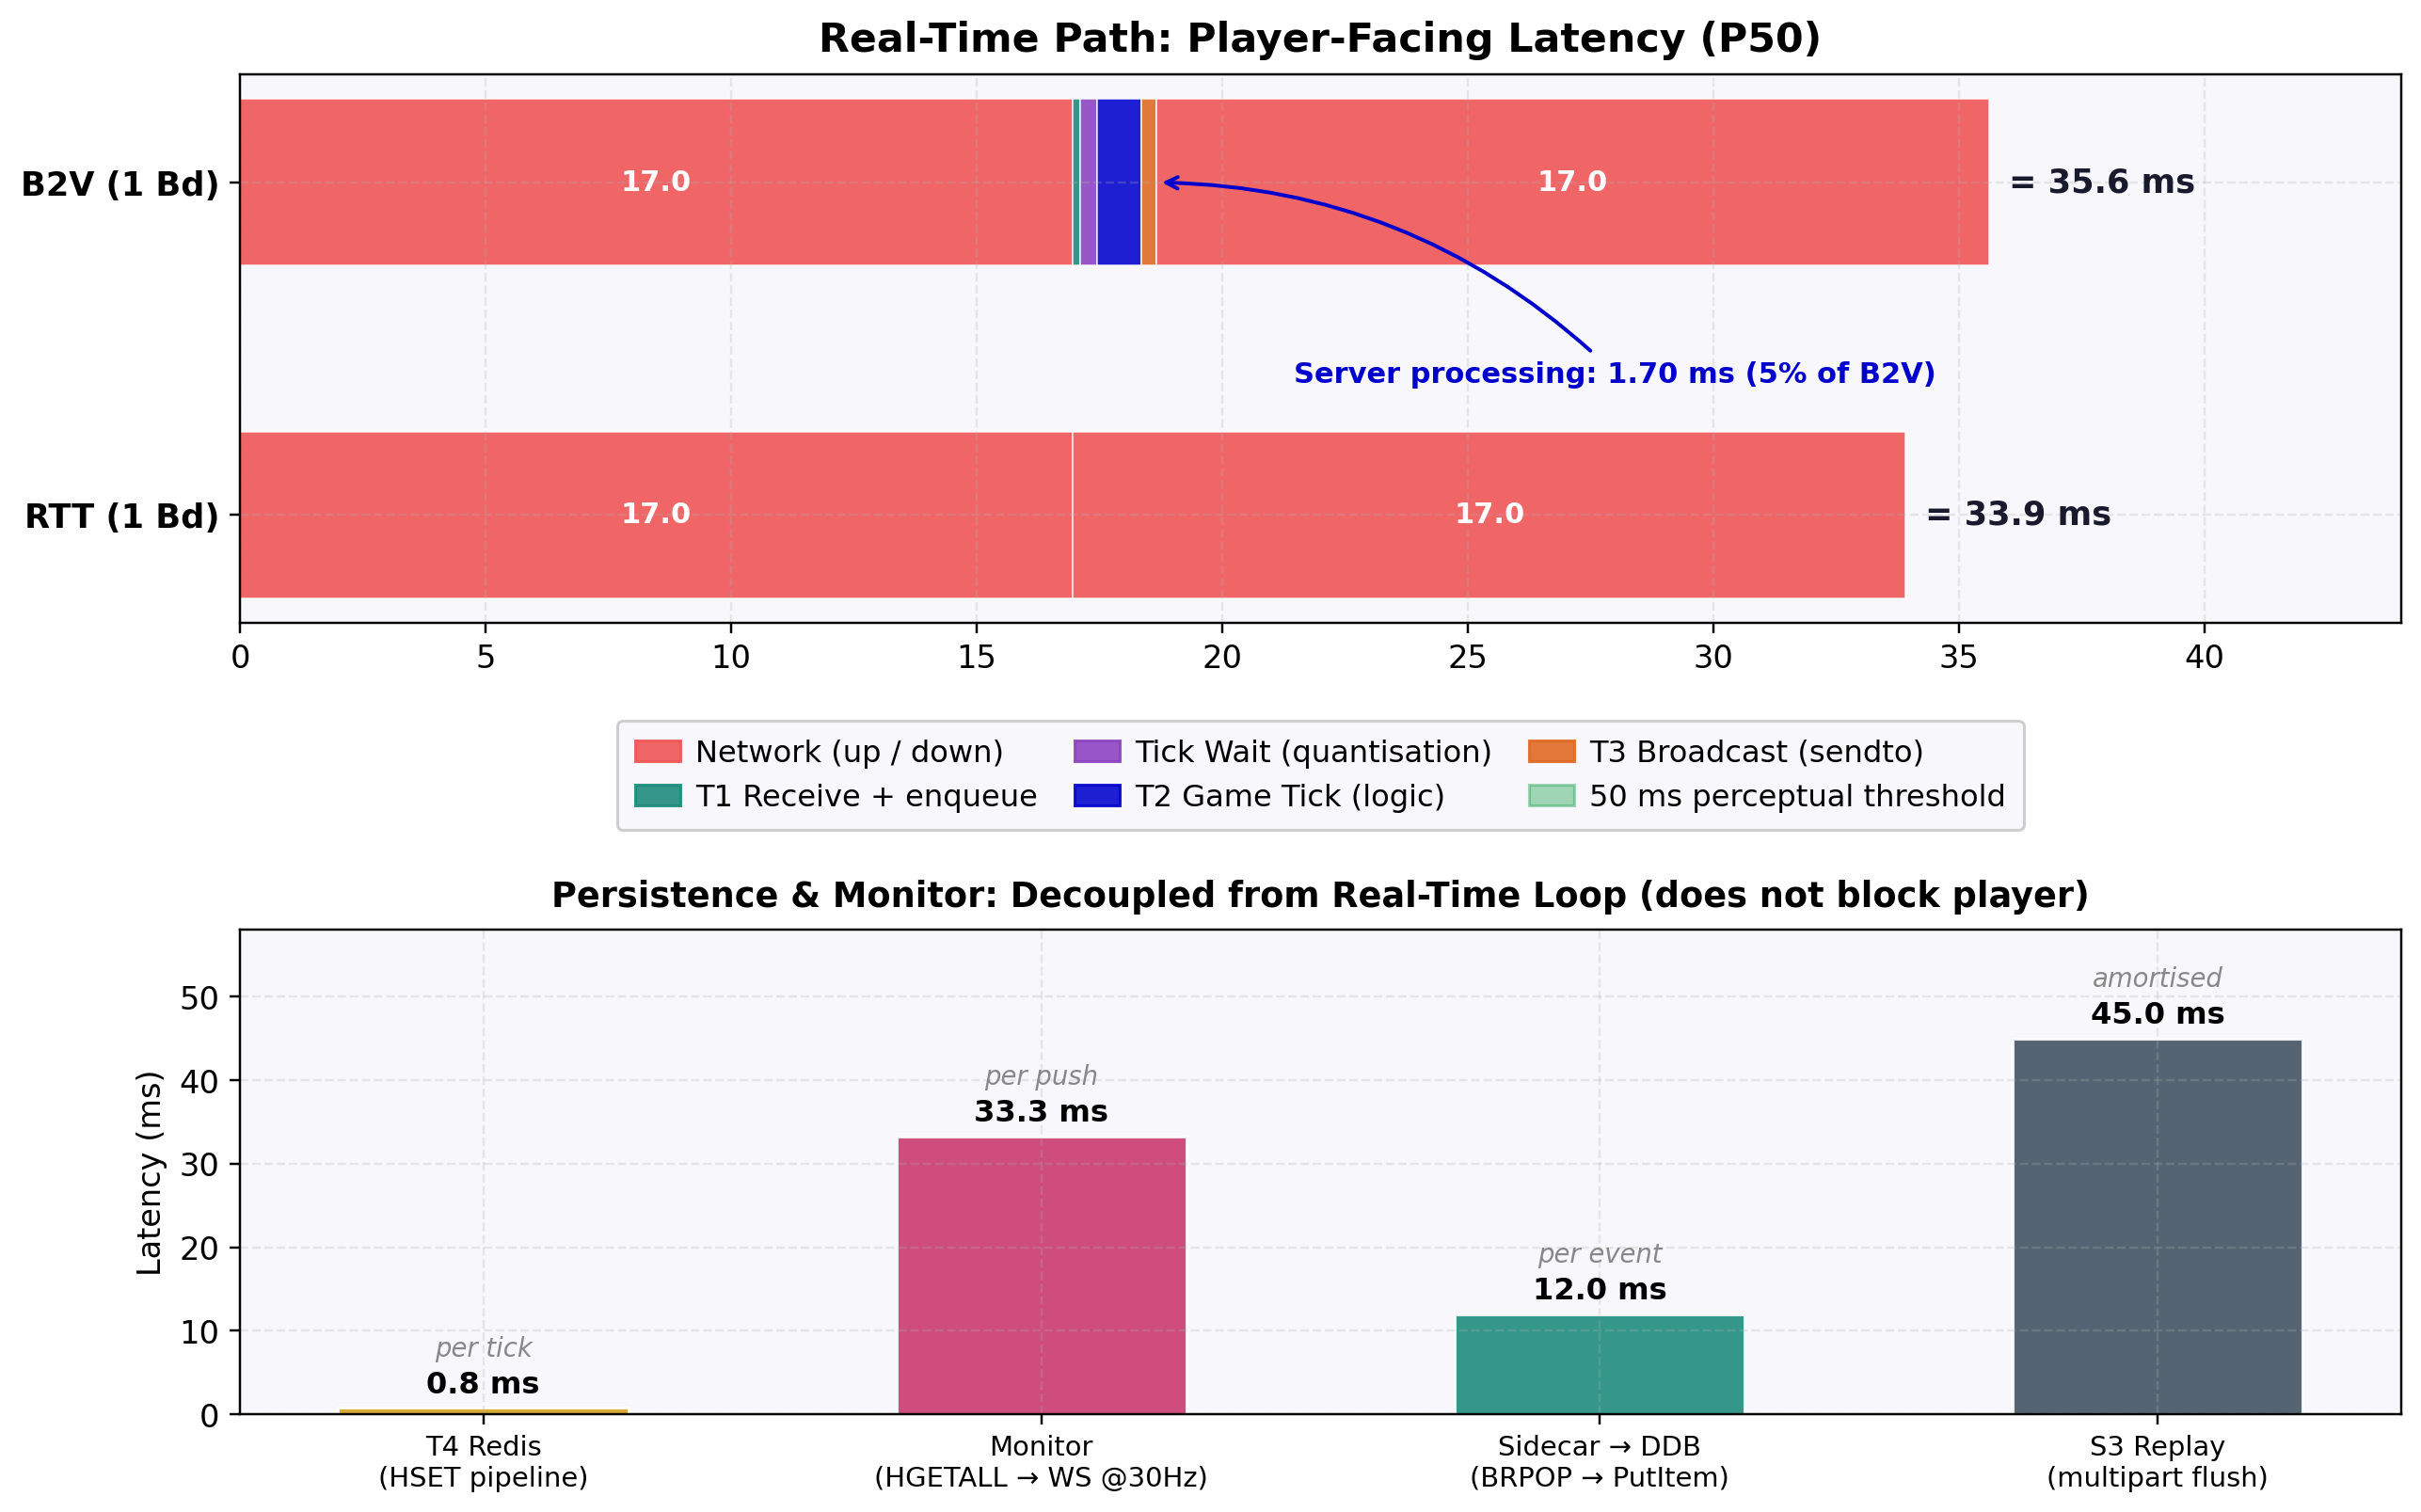
\includegraphics[width=\linewidth]{images/latency_system.png}
  \caption{Latency budget. Top: player-facing path with server overhead at 5\%. Bottom: decoupled persistence and monitor I/O.}
  \label{fig:system-latency}
\end{figure}


%%%%%%
\vspace{-15pt}
%%%%%
Figure~\ref{fig:load} shows B2V under increasing load and shows that the server acts uniformly even with all environment variables in action.

\begin{figure}[H]
  \centering
  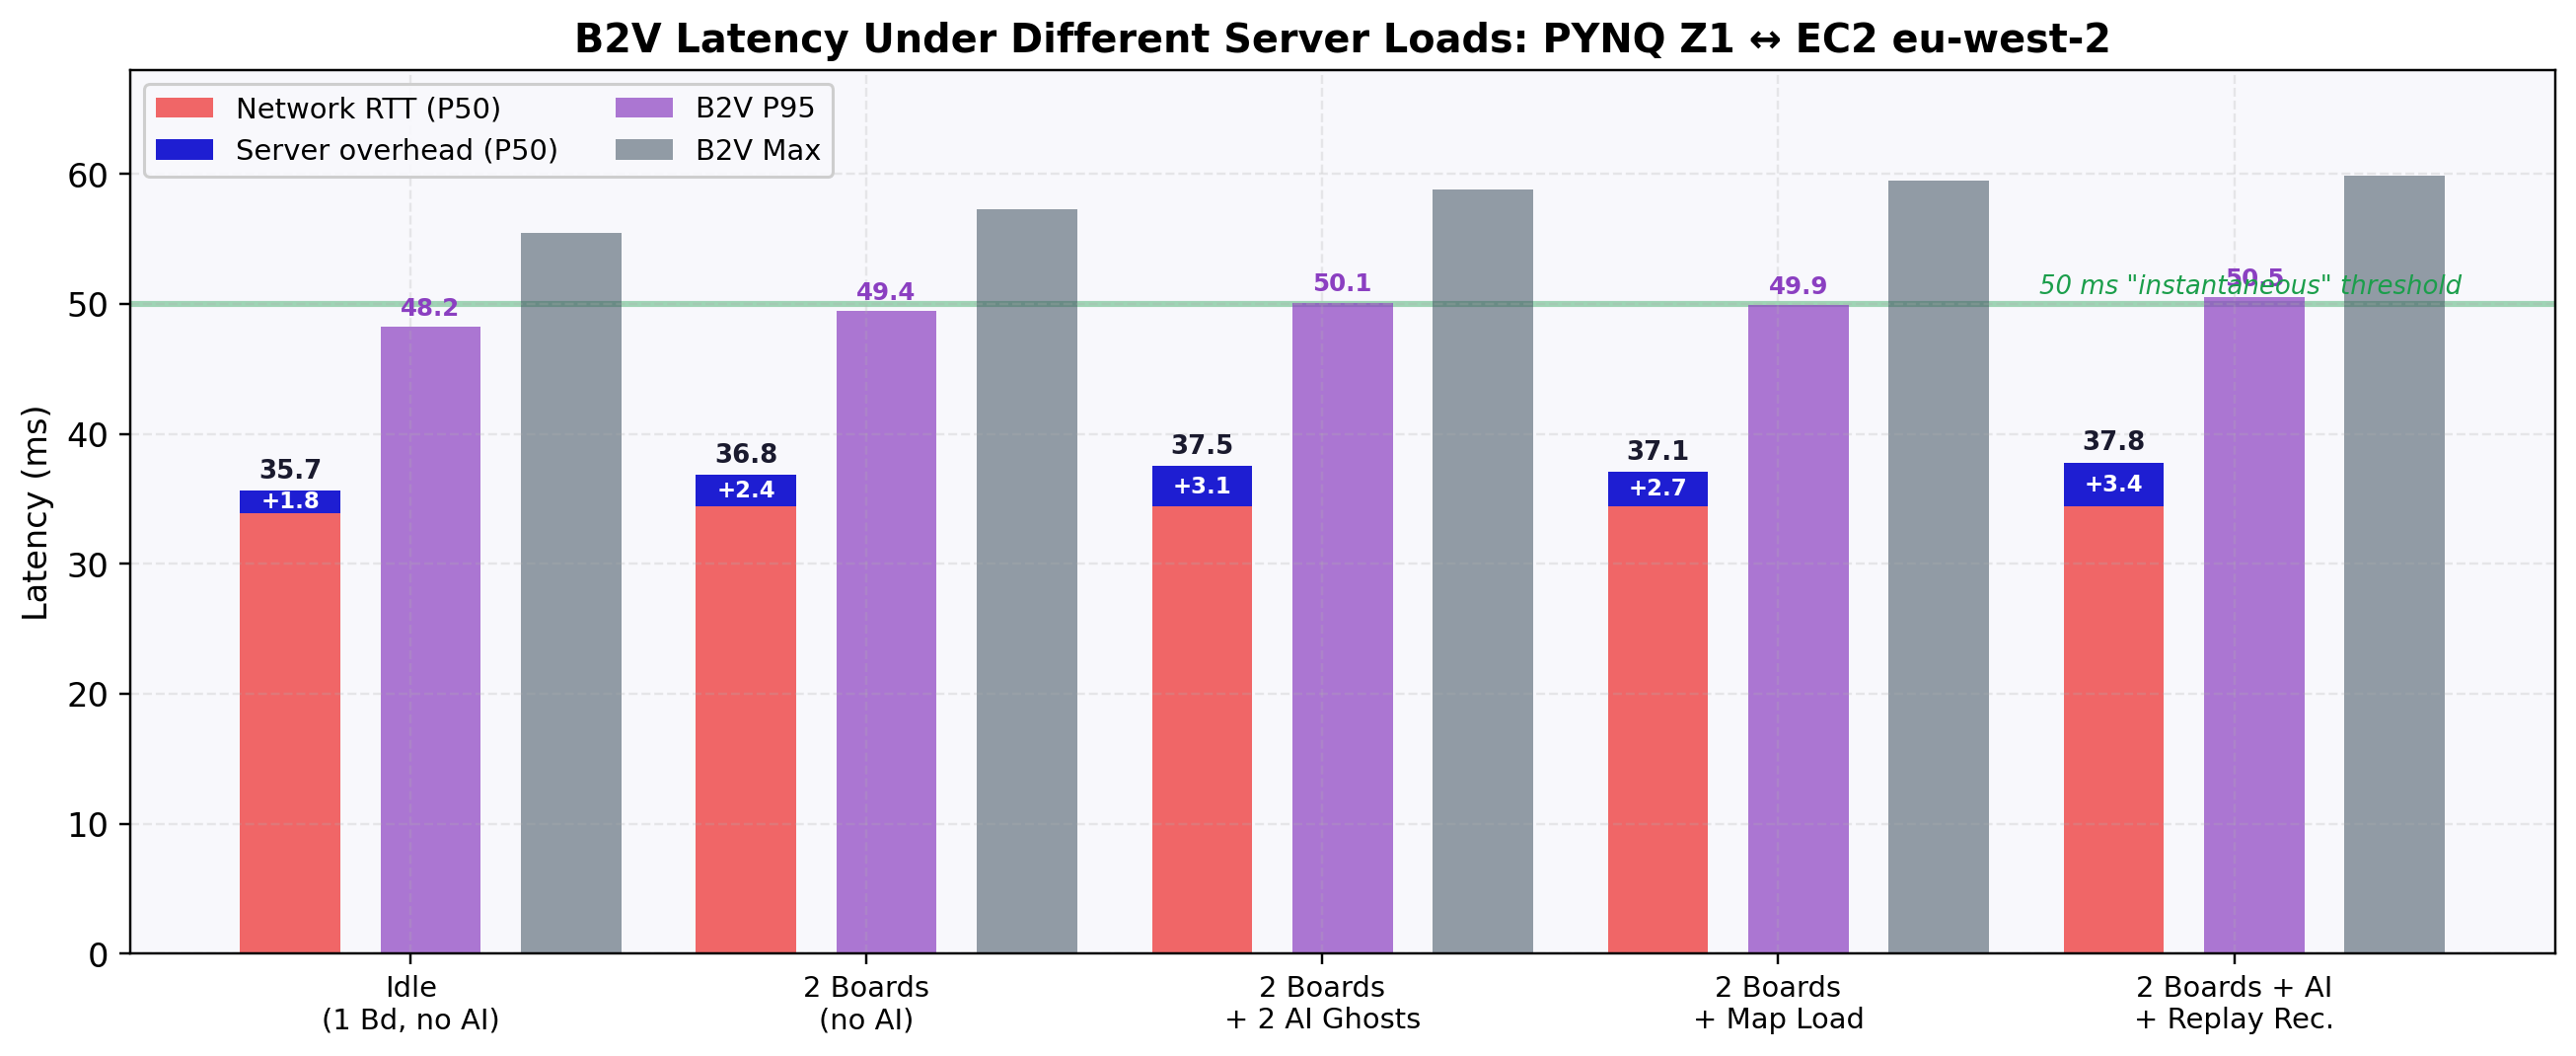
\includegraphics[width=\linewidth]{images/load_scenarios.png}
  \caption{B2V under load. Server overhead $<$4\,ms in all cases; P95 stays near 50\,ms.}
  \label{fig:load}
\end{figure}

Figure~\ref{fig:queues} shows the three inter-stage queue depths over 10\,s with 2~boards and 2~AI ghosts. All queues hover near zero (mean $<$0.5, max~4). No sustained growth confirms every stage drains faster than work arrives. This per-stage visibility is a direct benefit of the staged reactor topology, the queue-connected pipeline makes bottlenecks immediately attributable to a specific stage.

\begin{figure}[H]
  \centering
  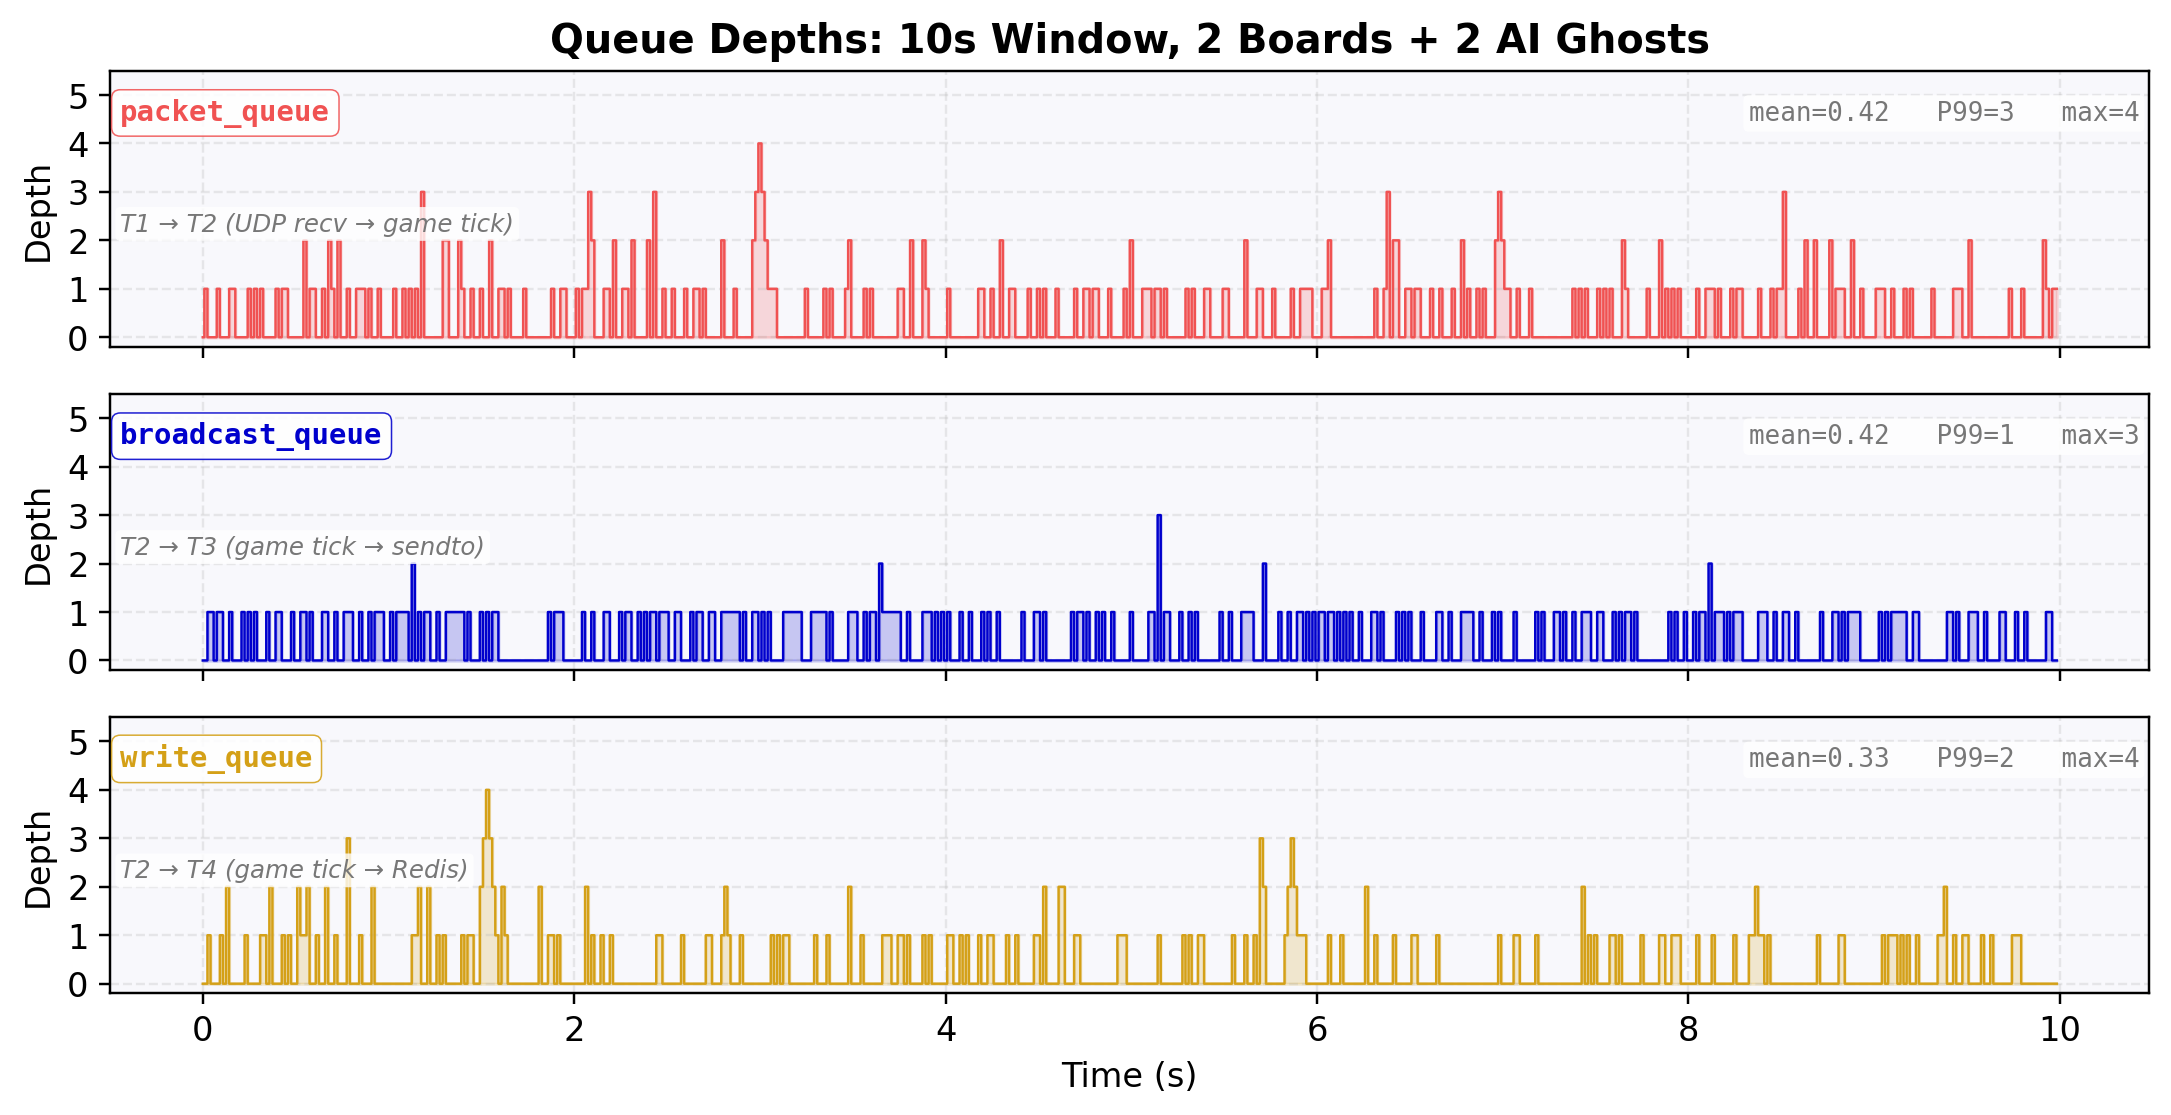
\includegraphics[width=\linewidth]{images/queue_depths.png}
  \caption{Queue depths: 10\,s, 2~boards + AI. Mean $<$0.5, no backpressure.}
  \label{fig:queues}
\end{figure}
